\documentclass{article}
\usepackage[utf8]{inputenc}
\usepackage{tikz}
\usepackage{float}

\title{ICSI412 Project 2: Documentation}
\author{Huang Kaisheng (2020215138@stu.cqupt.edu.cn)}
\date{May. 28th, 2023}

\begin{document}

\maketitle
\newpage

\tableofcontents
\newpage


\section{System Documentation}
This section contains a high-level data flow diagram, list of routines and brief descriptions and some implementation details.
\subsection{High-level Data Flow Diagram}
Figure \ref{dataflowdiagram} shows the high level data flow diagram.
\begin{figure}[H]

\begin{tikzpicture}[node distance=2cm]
\usetikzlibrary{shapes.geometric, arrows}

\tikzstyle{process} = [rectangle, rounded corners, minimum width=3cm, minimum height=1cm,text centered, draw=black, fill=red!30]
\tikzstyle{thread} = [rectangle, minimum width=3cm, minimum height=1cm, text centered, text width=3cm, draw=black, fill=orange!30]
\tikzstyle{io} = [trapezium, trapezium left angle=70, trapezium right angle=110, minimum width=1cm, minimum height=1cm, text centered, draw=black, fill=blue!30]
\tikzstyle{arrow} = [thick,->,>=stealth]
\tikzstyle{owned} = [thin,->,>=stealth]
\tikzstyle{ioarrow} = [dashed,->,>=stealth]

\node (stdin) [io, above of=consumer, xshift=0cm] {Standard Input};
\node (stdout) [io, above of=consumer, xshift=6cm] {Standard Output};

\node (producer) [process] {Producer};
\node (consumer) [process, right of=producer, xshift=5cm] {Consumer};


\node (reader) [thread, below of=producer] {Reader Thread};
\node (character) [thread, below of=reader] {Character Thread};
\node (toupper) [thread, below of=character] {ToUpper Thread};
\node (writer) [thread, below of=toupper] {Writer Thread};

\node (result) [io, right of=writer, xshift=3cm] {Result File};

\draw [ioarrow] (stdin) -- (consumer);
\draw [ioarrow] (consumer) -- (stdout);
\draw [dashed] (consumer) -- (producer);
\draw [owned] (producer) -- (reader);
\draw [arrow] (reader) -- (character);
\draw [arrow] (character) -- (toupper);
\draw [arrow] (toupper) -- (writer);
\draw [ioarrow] (writer) -- (result);
\draw [ioarrow] (result) -- (consumer);

\end{tikzpicture}
\caption{Data Flow Diagram}\label{dataflowdiagram}
\end{figure}

\subsection{List of Routines and Brief Descriptions}
\begin{center}
\begin{tabular}{|p{4cm}|p{7cm}|}
\hline
\textbf{Function} & \textbf{Description} \\ \hline
\texttt{mq\_initialize} & Initializes a message queue structure with mutex and head and tail node pointers set to NULL.\\ \hline
\texttt{mq\_push} & Adds a message to the tail of the message queue, allocating memory for a new node and copying the message into the node's buffer. Returns an error if the message size exceeds \texttt{MQ\_BUFFER\_SIZE}. \\ \hline
\texttt{mq\_pop} & Removes a message from the head of the message queue, copying it to the specified destination buffer and freeing the corresponding node's memory. Returns an error if the message queue is empty or the specified size is less than the message buffer size. \\ \hline
\texttt{mq\_destroy} & Frees all memory used by the message queue structure and destroys the mutex. \\ \hline
\texttt{\_try} & Executes an expression and checks the return value. If the return value is non-zero, prints an error message and exits the program. \\ \hline
\texttt{\_try\_do} & Executes an expression and checks the return value. If the return value is non-zero, prints an error message. Otherwise, executes a specified command. \\ \hline
\texttt{debug} & Prints a debug message to the standard error stream if the DEBUG macro is defined. \\ \hline
\texttt{readerFunc} & Reads from a file and adds each line to a message queue. \\ \hline
\texttt{characterFunc} & Replaces spaces, tabs, and newlines in messages with a specified character. \\ \hline
\texttt{toUpperFunc} & Converts all lowercase alphabetical characters in messages to uppercase. \\ \hline
\texttt{writerFunc} & Writes each message to a file, adding a newline character after each message. \\ \hline
\texttt{main} (in \texttt{producer.c}) & Initializes semaphores and message queues, creates threads for each function, joins the threads, and destroys the semaphores and message queues. \\ \hline
\texttt{main} (in \texttt{consumer.c}) & Prompts the user to enter a filename, location, and character, creates a child process to execute the producer program, reads the filename of the result file from a pipe, opens the result file, reads and prints each line of the result file, and deletes the result file. \\ \hline
\end{tabular}
\end{center}
\newpage

\subsection{List of Semaphores, Mutexes and Their Descriptions}
\subsubsection{Semaphores}
\begin{center}
\begin{tabular}{|p{4cm}|p{7cm}|}
\hline
\textbf{Semaphore} & \textbf{Description} \\ \hline
\texttt{semReaderToCharacter} & Controls the synchronization between the reader thread and the character thread by signaling the latter thread when there is new input available. \\ \hline
\texttt{semCharacterToToUpper} & Controls the synchronization between the character thread and the toUpper thread by signaling the latter thread when there are new character modifications available. \\ \hline
\texttt{semToUpperToWriter} & Controls the synchronization between the toUpper thread and the writer thread by signaling the latter thread when there is new output available. \\
\hline
\end{tabular}
\end{center}

\subsubsection{Mutexes}
\begin{center}
\begin{tabular}{|p{4cm}|p{7cm}|}
\hline
\textbf{Mutex} & \textbf{Description} \\ \hline
\texttt{message\_queue::mutex} & Protects the access of the message queue by controlling the mutual exclusion of multiple threads attempting to modify the queue simultaneously. \\ 
\hline
\end{tabular}
\end{center}

\subsection{Implementation Details}
The project shown above is a consumer-producer pair which reads a text file and transform its content concurrently.

The project consists of two programs: \texttt{producer.c} and \texttt{consumer.c}. The \texttt{producer.c} program reads from a file, performs character substitution and uppercase transformation, and writes the result to a new file. The \texttt{consumer.c} program prompts the user for a file name, location, and character to substitute, executes \texttt{producer.c} as a child process using \texttt{fork}, reads the result file produced by \texttt{producer.c}, and prints the contents to standard output.

The \texttt{producer.c} program has four threads: \texttt{reader}, \texttt{character}, \texttt{toUpper}, and \texttt{writer}. The \texttt{reader} thread reads from a file specified by the second argument passed on the command line, and pushes each line of the file onto a message queue called \texttt{readerToCharacter}. The \texttt{character} thread pops each line from \texttt{readerToCharacter}, performs character substitution based on a character specified by the third argument passed on the command line, and pushes each transformed line onto a message queue called \texttt{characterToToUpper}. The \texttt{toUpper} thread pops each line from \texttt{characterToToUpper}, performs uppercase transformation, and pushes each transformed line onto a message queue called \texttt{toUpperToWriter}. The \texttt{writer} thread pops each line from \texttt{toUpperToWriter} and writes it to a file specified by the first argument passed on the command line. The \texttt{writer} thread also prints the path of the new file to standard output. Each thread is implemented as a function that takes a \texttt{void*} argument and returns a \texttt{void*} argument.

The \texttt{message\_queue} module provides a message queue data structure, which is used to pass messages between threads. The message queue is implemented as a singly-linked list of \texttt{message\_queue\_node} structures. Each node contains a message buffer and the size of the message. The message queue provides three functions: \texttt{mq\_initialize} to initialize the message queue; \texttt{mq\_push} to push a message onto the queue; and \texttt{mq\_pop} to pop a message from the queue. The \texttt{mq\_initialize} function initializes the mutex used to provide thread safety. The \texttt{mq\_push} function creates a new node for the message and appends it to the end of the queue. The \texttt{mq\_pop} function removes the first node from the queue and returns the message buffer.

The \texttt{consumer.c} program prompts the user for a file name, location, and character to replace. It then creates a pipe using the \texttt{pipe} system call and forks a child process using the \texttt{fork} system call. The child process executes \texttt{producer.c} with the specified command-line arguments and writes the resulting file name to the pipe. The parent process reads the file name from the pipe, reads the contents of the resulting file, and prints the contents to standard output. The parent process also removes the resulting file using the \texttt{remove} system call.

The \texttt{macros.h} header file provides several macros used throughout the project. The \texttt{\_try} macro is used to check the return value of a function call for errors and prints an error message if the return value is non-zero. The \texttt{\_try\_do} macro is similar to \texttt{\_try}, but allows the user to specify an additional statement to execute if the function call succeeds. The \texttt{debug} macro is used to print debug messages to standard error. If the \texttt{DEBUG} macro is defined at compile time, debug messages are printed; otherwise, they are ignored.

Overall, the project demonstrates the use of threads, message passing using a message queue, system calls (\texttt{fork}, \texttt{pipe}, \texttt{execlp}, \texttt{fclose}, \texttt{fopen}), and file I/O in C. The modular structure of the project separates the message queue implementation from the producer/consumer logic, making the code more maintainable and easier to understand.

\section{Test Documentation}
This section contains the description of test method, and a test result.
\subsection{Test Method}
\subsubsection{Unit Test}
For the message queue module, I wrote a unit test driver to test its thread safety and correctness, whose procedure is: \\
1. Enter \texttt{unit-test} directory \\
2. Run \texttt{make} to build and run the test. \\
3. Observe the result. \\

\subsubsection{Full-featured Test}
To test the full feature, I copied a piece of lyric from a popular song \textit{The Rose} by \textit{Amanda McBrooms}. We should first build the program and let consumer to ask the producer. Procedure is: \\
1. Run \texttt{make} to build. \\
2. Run \texttt{./consumer} to start the consumer program \\
3. Give it the information of our test suite. \\
4. Observe the result. \\

\subsection{Test Result}
\subsubsection{Unit Test}
Let's see the result:
\begin{verbatim}
victor@victor-dev:~/CSI412/Project2/unit-test(master○) » make
make message_queue_test
make[1]: Entering directory '/home/victor/CSI412/Project2/unit-test'
gcc -c -o message_queue_test.o message_queue_test.c -I.. -lpthread
gcc -c -o ../message_queue.o ../message_queue.c -I.. -lpthread
gcc -o message_queue_test message_queue_test.o ../message_queue.o -I.. -lpthread
make[1]: Leaving directory '/home/victor/CSI412/Project2/unit-test'
bash -c '(diff -w <(./message_queue_test) message_queue_test.out &&
echo "✅ TEST PASSED") || (echo "❌ TEST FAILED")'
mq_initialize: 0
thread 3: mq_push: 0
thread 2: mq_push: 0
thread 3: mq_pop: 0
thread 2: mq_pop: 0
thread 1: mq_push: 0
thread 1: mq_pop: 0
mq_destroy: 0
✅ TEST PASSED
\end{verbatim}
\subsubsection{Full-featured Test}

With the test suite I mentioned before:
\begin{verbatim}
victor@victor-dev:~/CSI412/Project2(master○) » ./consumer                                   
Enter file name: rose.txt
Enter file location: ./testdata/rose.txt
Enter character: _
Acknowledged result file: /tmp/proj2.uXGSa4/rose.txt

SOME_SAY,_"LOVE,_IT_IS_A_RIVER_
THAT_DROWNS_THE_TENDER_REED"_
SOME_SAY,_"LOVE,_IT_IS_A_RAZOR_
THAT_LEAVES_YOUR_SOUL_TO_BLEED"_
SOME_SAY,_"LOVE,_IT_IS_A_A_HUNGER_
AN_ENDLESS_ACHING_NEED"_
I_SAY,_"LOVE,_IT_IS_A_FLOWER_
AND_YOU_IT'S_ONLY_SEED"_
\end{verbatim}

The content of test suite \texttt{rose.txt}:
\begin{verbatim}
Some say, "Love, it is a river
That drowns the tender reed"
Some say, "Love, it is a razor
That leaves your soul to bleed"
Some say, "Love, it is a a hunger
An endless aching need"
I say, "Love, it is a flower
And you it's only seed"
\end{verbatim}

\subsubsection{Running Screenshot}

\begin{figure}[H]
    \centering
    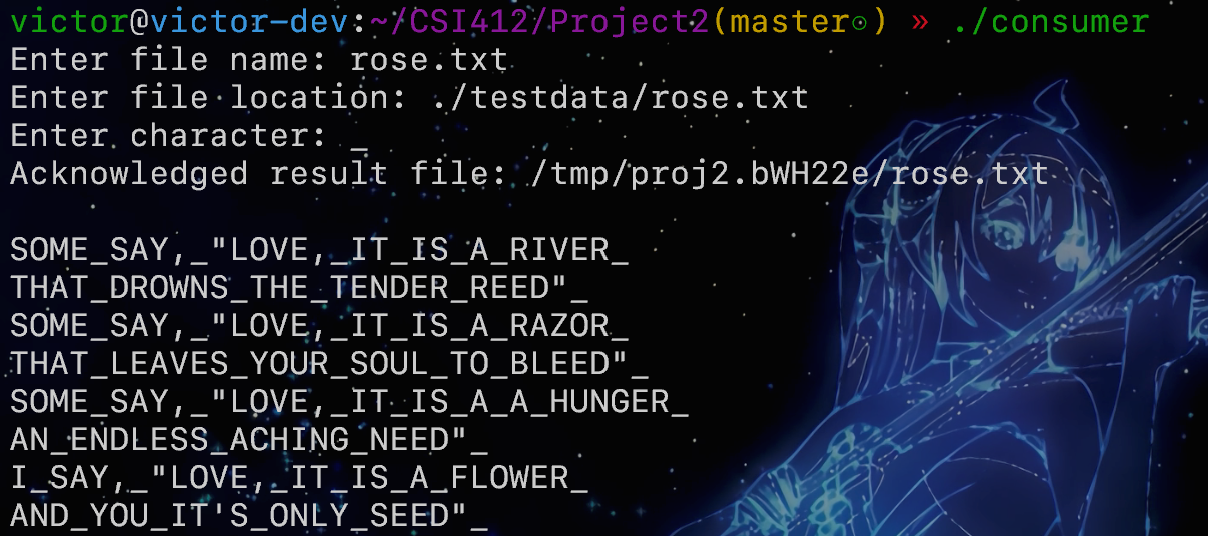
\includegraphics[width=15cm, screenshot]{img/project2_run_result.png}
    \caption{The screenshot of the project}
\end{figure}

\subsection{Known Bugs and Plans to Address}
\subsubsection{Known Bugs}
We currently do not have enough error handling. 

If user provide a not existed file location, the producer cannot tell the consumer, which can lead to undefined behaviors.

And any errors occur in threads may cause the producer into undefined state.

\subsubsection{Plans to Address}
These bugs can be fixed theoretically by: \\
1. Implement structured pipe communication, instead of using pure filename output. \\
2. Make retrying mechanism inside the thread. If necessary, panic the full process.\\

\section{User Documentation}
This section contains how to build the program and argument definition.

\subsection{How to run the program}
Make sure that there is a C compiler and GNU make in your environment. \\
Run \texttt{make} to compile the programs. \\
And the binaries will appear at \texttt{consumer} and \texttt{producer}.

\subsection{Argument Definition}
For the two programs:

The consumer does not receive any arguments. It prompts and read information from standard input.

The producer receives 3 required arguments. The usage is:
\begin{verbatim}
./producer <file name> <file location> <character to replace>
\end{verbatim}

The producer should not be directly run, it should be run by consumer.
\end{document}
